\documentclass[10pt]{article}

\usepackage[a4paper,margin=0.78in]{geometry}
\usepackage{amsmath,amssymb}
\usepackage{booktabs}
\usepackage{enumitem}
\usepackage{graphicx}
\usepackage{listings}
\usepackage{xcolor}
\usepackage{microtype}
\usepackage{natbib}
\usepackage{url}
\usepackage[colorlinks=true,allcolors=blue!55!black]{hyperref}

\newcommand{\tespec}{\textsc{TeSpec}}
\newcommand{\qcp}{\textsc{QCP}}
\newcommand{\rocq}{Rocq}
\newcommand{\pass}{\textsf{SATISFIED}}
\newcommand{\fail}{\textsf{VIOLATED}}
\newcommand{\unknown}{\textsf{UNKNOWN}}
\newcommand{\manual}{\textsf{RESIDUAL}}

\lstdefinelanguage{QCP}{
  language=C,
  morekeywords={With,Require,Ensure,Let,Extern,Coq,Import,exists,forall},
  sensitive=true
}
\lstset{
  language=QCP,
  basicstyle=\ttfamily\small,
  keywordstyle=\color{blue!65!black}\bfseries,
  commentstyle=\color{green!35!black},
  numbers=left,
  numberstyle=\scriptsize\color{gray},
  frame=single,
  breaklines=true,
  columns=fullflexible,
  xleftmargin=1.5em,
  framexleftmargin=1em
}

\title{\textsc{TeSpec}: Proof-Backed Instance Testing of\\
C Heap Specifications}
\author{Anonymous Authors}
\date{}

\begin{document}
\maketitle

\begin{abstract}
Formal specifications are increasingly generated by automated tools and large
language models, yet checking whether a generated specification captures the
intended behavior remains difficult.  Runtime checking and property-based
testing now support substantial fragments of separation logic, including
complex C heaps, but rely on contracts with a supplied computational
interpretation.  At the same time, specification-evaluation systems can prove
declarative propositions on concrete value-level examples.  Our target lies
between these lines: existing QCP contracts that combine mutable C heaps with
ghost values, quantifiers, and application-specific Rocq propositions for
which no runtime monitor has been supplied.

We present \tespec, a proof-backed specification-testing tool for QCP-annotated
C functions.  Its input is a C implementation and contract together with typed
bindings for C parameters and logical \texttt{With} variables.  Instead of
compiling a second executable oracle, \tespec{} follows the concrete
program path in a modified QCP symbolic executor, directly executes finite
loops and visible calls, and specializes the original pre/postcondition with
the observed heap transition.  QCP and SMT discharge routine obligations;
unresolved formulas remain visible Rocq goals that may be completed by a human
or proof agent.  The deterministic core, rather than the agent, checks all
inputs and evidence.

Through a running minimum-subarray example, we show how one test simultaneously
fixes C arguments, a concrete array heap, and its logical list view, and how a
proof-oriented postcondition becomes a closed proposition about the observed
return and final heap.  \tespec{} is not a replacement for universal
verification: it provides reproducible evidence about selected concrete heap
behaviors without requiring the original contract to be rewritten as a
runtime checker.
\end{abstract}

\section{Introduction}

Formal verification establishes that an implementation satisfies a
specification, but does not establish that the specification expresses what a
developer intended.  This familiar oracle problem has become more visible as
large language models (LLMs) are used to generate preconditions,
postconditions, invariants, and auxiliary predicates.  A generated contract can
parse, type-check, and even verify while remaining vacuous, incomplete, or
semantically misaligned.

Specification evaluation has therefore become an independent software
engineering problem.  FormalBench evaluates inferred specifications using
consistency and completeness checks~\citep{lecong2025formalbench}.  CLEVER
uses formal equivalence to curated references~\citep{thakur2025clever}.
VERINA separates code, specification, and proof generation and uses positive
and negative examples to evaluate specification quality~\citep{ye2026verina}.
COINS specializes declarative Rocq propositions to concrete input/output pairs
and asks a proof checker to validate the resulting instances
~\citep{yang2026coins}.  These approaches avoid relying solely on whether one
implementation verifies, but their examples are predominantly relations over
ordinary values.

Property-based testing (PBT) attacks a closely related problem from the testing
side.  QuickCheck repeatedly evaluates an executable property on generated
inputs; QuickChick brings this workflow to Coq, and FuzzChick improves input
exploration with coverage guidance~\citep{claessen2000quickcheck,
paraskevopoulou2015quickchick,
lampropoulos2019fuzzchick}.  For heap-manipulating C, Fulminate instruments CN
contracts with runtime ownership checks, while Bennet synthesizes randomized
heap generators from the restricted CN separation-logic fragment
~\citep{banerjee2025fulminate,aamer2025bennet}.  These systems demonstrate that
heap-aware specification testing is both feasible and useful.  Their runtime
approach deliberately relies on a specification fragment with a predictable
computational interpretation.

QCP occupies a different point in the design space.  Its contracts may use
separating conjunction, recursive predicates, quantifiers, arbitrary
\texttt{With} types, old-state values, and imported Rocq definitions
~\citep{wu2026qcp}.  This expressiveness is useful for verification but does
not by itself provide a runtime interpretation.  Some QCP spatial predicates,
such as arrays and input-directed lists, clearly admit monitors; others invoke
application-specific Rocq propositions that would first have to be translated
into decision procedures.  Doing so manually duplicates the oracle and creates
a new equivalence obligation between the monitor and the contract.

This paper explores a pragmatic alternative:

\begin{quote}
\emph{Can we obtain useful test feedback for proof-oriented C heap contracts
without first rewriting them as executable properties?}
\end{quote}

We implement this idea in \tespec.  A test case supplies concrete C inputs,
heap data, and typed values for the contract's logical variables.  A modified
QCP executor follows the selected execution, unrolling finite loops and
entering visible callees instead of asking for loop invariants and callee
contracts.  At function return, the tool substitutes the initial and final
states into the original \texttt{Require}/\texttt{Ensure}, simplifies closed
operations, and invokes the ordinary QCP/Rocq proof pipeline.  A proof-backed
success is conclusive for that instance; an unresolved goal is reported rather
than silently accepted.

The approach resembles PBT in its use of concrete cases and fast feedback, but
differs in its oracle: the property need not arrive with an executable decision
procedure.  It resembles
instance-based specification evaluation, but the observed behavior is a
mutable heap transition rather than an immutable pair.  It complements
Fulminate and Bennet by trading randomized runtime throughput for a wider
assertion language and proof-producing residual path.

This paper makes the following software-engineering contributions:

\begin{enumerate}[leftmargin=1.4em]
  \item We formulate testing a QCP contract as proof checking over an indexed
        concrete heap transition, preserving the original assertion as the
        oracle.
  \item We introduce a practical interface for supplying typed C inputs, heap
        descriptions, and logical-variable bindings without encoding expected
        outputs in an executable test harness.
  \item We adapt QCP symbolic execution to follow finite concrete loops and
        visible calls without requiring test authors to write invariants or
        callee specifications for the selected case.
  \item We combine generic closed-term simplification, QCP/SMT automation, and
        residual Rocq proofs in a transparent evidence workflow whose optional
        agent layer cannot determine verdicts by itself.
\end{enumerate}

We deliberately do not claim that passing finitely many cases proves a
contract universally correct.  \tespec{} is a specification-testing and
debugging tool: it supplies machine-checked evidence for selected behaviors
and makes unsupported or unresolved cases explicit.

\section{Motivating Example}
\label{sec:motivation}

\subsection{A proof-oriented contract over a C heap}

We begin with a small but representative function adapted from our subject
corpus.  It reads a heap-resident array and returns the minimum sum of any
nonempty contiguous subarray.  Its QCP contract connects three views of the
same input: the C pointer and length, a logical list \texttt{nums\_l}, and the
bytes owned by the array predicate.

\begin{lstlisting}
/* abridged from the artifact case */
/*@ Extern Coq
      (problem_114_spec : list Z -> Z -> Prop)
      (kadane_int64_range : list Z -> Prop) */
long long p114_minSubArraySum(long long *nums, int nums_size)
/*@ With (nums_l : list Z)
    Require
      1 <= nums_size &&
      nums_size == Zlength(nums_l) &&
      kadane_int64_range(nums_l) &&
      LongArray::full(nums, nums_size, nums_l)
    Ensure
      problem_114_spec(nums_l, __return) &&
      LongArray::full(nums, nums_size, nums_l)
*/
{
  long long cur = nums[0], best = nums[0];
  for (int i = 1; i < nums_size; ++i) {
    cur = cur < 0 ? cur + nums[i] : nums[i];
    if (cur < best) best = cur;
  }
  return best;
}
\end{lstlisting}

The imported Rocq proposition is intentionally declarative.  Omitting minor
library syntax, it says
\[
\begin{split}
\mathsf{MinSpec}(xs,r) \triangleq {}&
  \bigl(\exists pre,seg,suf.\;seg\neq[] \land
        xs=pre\mathbin{++}seg\mathbin{++}suf \land
        \mathsf{sum}(seg)=r\bigr) \\
&{}\land
  \bigl(\forall pre,seg,suf.\;seg\neq[] \land
        xs=pre\mathbin{++}seg\mathbin{++}suf
        \Rightarrow r\leq\mathsf{sum}(seg)\bigr).
\end{split}
\]
The first conjunct requires a witness attaining \(r\); the second states
minimality over all subarrays.  This is ordinary proof-oriented Rocq:
\texttt{problem\_114\_spec} has type \texttt{Prop}, contains nested
quantification over lists, and is imported as a logical definition rather than
as a Boolean procedure.

The heap is not, by itself, the obstacle.  A monitor can walk
\texttt{LongArray::full(nums,nums\_size,nums\_l)}, check allocation and
ownership, and compare the six cells with \texttt{nums\_l}.  Fulminate gives
precisely this kind of computational interpretation to CN resources, and
Bennet runs the interpretation in reverse to generate satisfying
heaps~\citep{banerjee2025fulminate,aamer2025bennet}.  The missing component is
a monitor for the imported \(\mathsf{MinSpec}\).  It is decidable for a finite
list, but the QCP source supplies no decision procedure.  A user could write
one, but would then have to maintain a second oracle and justify that it is
equivalent to the Rocq proposition.

\subsection{One indexed heap behavior}

A \tespec{} case makes the pre-state explicit:

\begin{lstlisting}
{
  "args":   {"nums": 12288, "nums_size": 6},
  "values": {"nums_l": [2, 3, 4, 1, 2, 4]}
}
\end{lstlisting}

The binding does not provide an expected return.  It states that address
\texttt{12288} is the root of a six-element array whose logical view is the
given list.  The spatial precondition materializes the corresponding typed
heap.  Concrete execution then follows five loop iterations:

\begin{center}
\small
\begin{tabular}{crrr}
\toprule
step & current element & \texttt{cur} & \texttt{best}\\
\midrule
entry & 2 & 2 & 2\\
1 & 3 & 3 & 2\\
2 & 4 & 4 & 2\\
3 & 1 & 1 & 1\\
4 & 2 & 2 & 1\\
5 & 4 & 4 & 1\\
\bottomrule
\end{tabular}
\end{center}

The observed behavior is
\[
  (\mathit{nums\_size}=6,\ H_0=[2,3,4,1,2,4])
  \longrightarrow
  (r=1,\ H_1=H_0).
\]
Substitution eliminates the C locals, loop path, pointer address, return
placeholder, and abstract pre-state variable.  The terminal contract becomes,
schematically,
\[
  \mathsf{MinSpec}([2,3,4,1,2,4],1)
  \;\land\;
  \mathsf{ArrayEq}(H_1,12288,[2,3,4,1,2,4]).
\]
The spatial conjunct is checked against the concrete final heap.  The first
conjunct is retained as a closed Rocq proposition: simplification may unfold
finite list operations, SMT may close arithmetic leaves, and any remaining
quantified reasoning is exported as a residual goal.  Failure to close that
goal yields \unknown{}, not a false counterexample.

\subsection{Why both positive and negative behaviors matter}

The example also shows why executing a correct implementation is insufficient
for evaluating specification quality.  Consider a plausible weakened
candidate that keeps only the existence conjunct of \(\mathsf{MinSpec}\).
It accepts the observed return \(1\), but it also accepts the invalid terminal
behavior \(r=2\), because the singleton subarray \([2]\) has sum \(2\).
Conversely, an over-strong candidate requiring \(r<0\) rejects the valid
behavior above.

\begin{center}
\small
\begin{tabular}{lcc}
\toprule
candidate contract & valid \(r=1\) & invalid \(r=2\)\\
\midrule
full existence-and-minimality relation & accept & reject\\
existence only & accept & accept\\
full relation plus \(r<0\) & reject & reject\\
\bottomrule
\end{tabular}
\end{center}

Positive heap executions therefore expose over-restriction, while frozen
negative terminal behaviors expose under-specification.  A strict semantic
rejection must be backed by a checked proof of the instantiated proposition's
negation; an execution error or failed proof search is not enough.

\subsection{The gap between existing approaches}

This example locates \tespec{} between two established workflows.  A
Bennet-style workflow can generate and execute rich C heaps when the complete
oracle is expressed in its deliberately executable CN fragment.  A
COINS-style workflow can instantiate a declarative proposition on a trusted
input/output pair, but its cases do not include a C execution with ownership,
aliasing, globals, and old/new heaps~\citep{yang2026coins}.  Universal QCP
verification preserves all of this state, but asks for the loop invariant and
proof needed for every legal input.

\tespec{} instead follows one finite C execution while retaining QCP's logical
heap and proof backend.  It neither claims Bennet's random generation
throughput nor COINS's language-independent value model.  Its intended use is
to test an existing proof-oriented C contract on selected heap behaviors
without first rewriting that contract into a separate executable property.

\section{Tool Overview}

\begin{figure}[t]
  \centering
  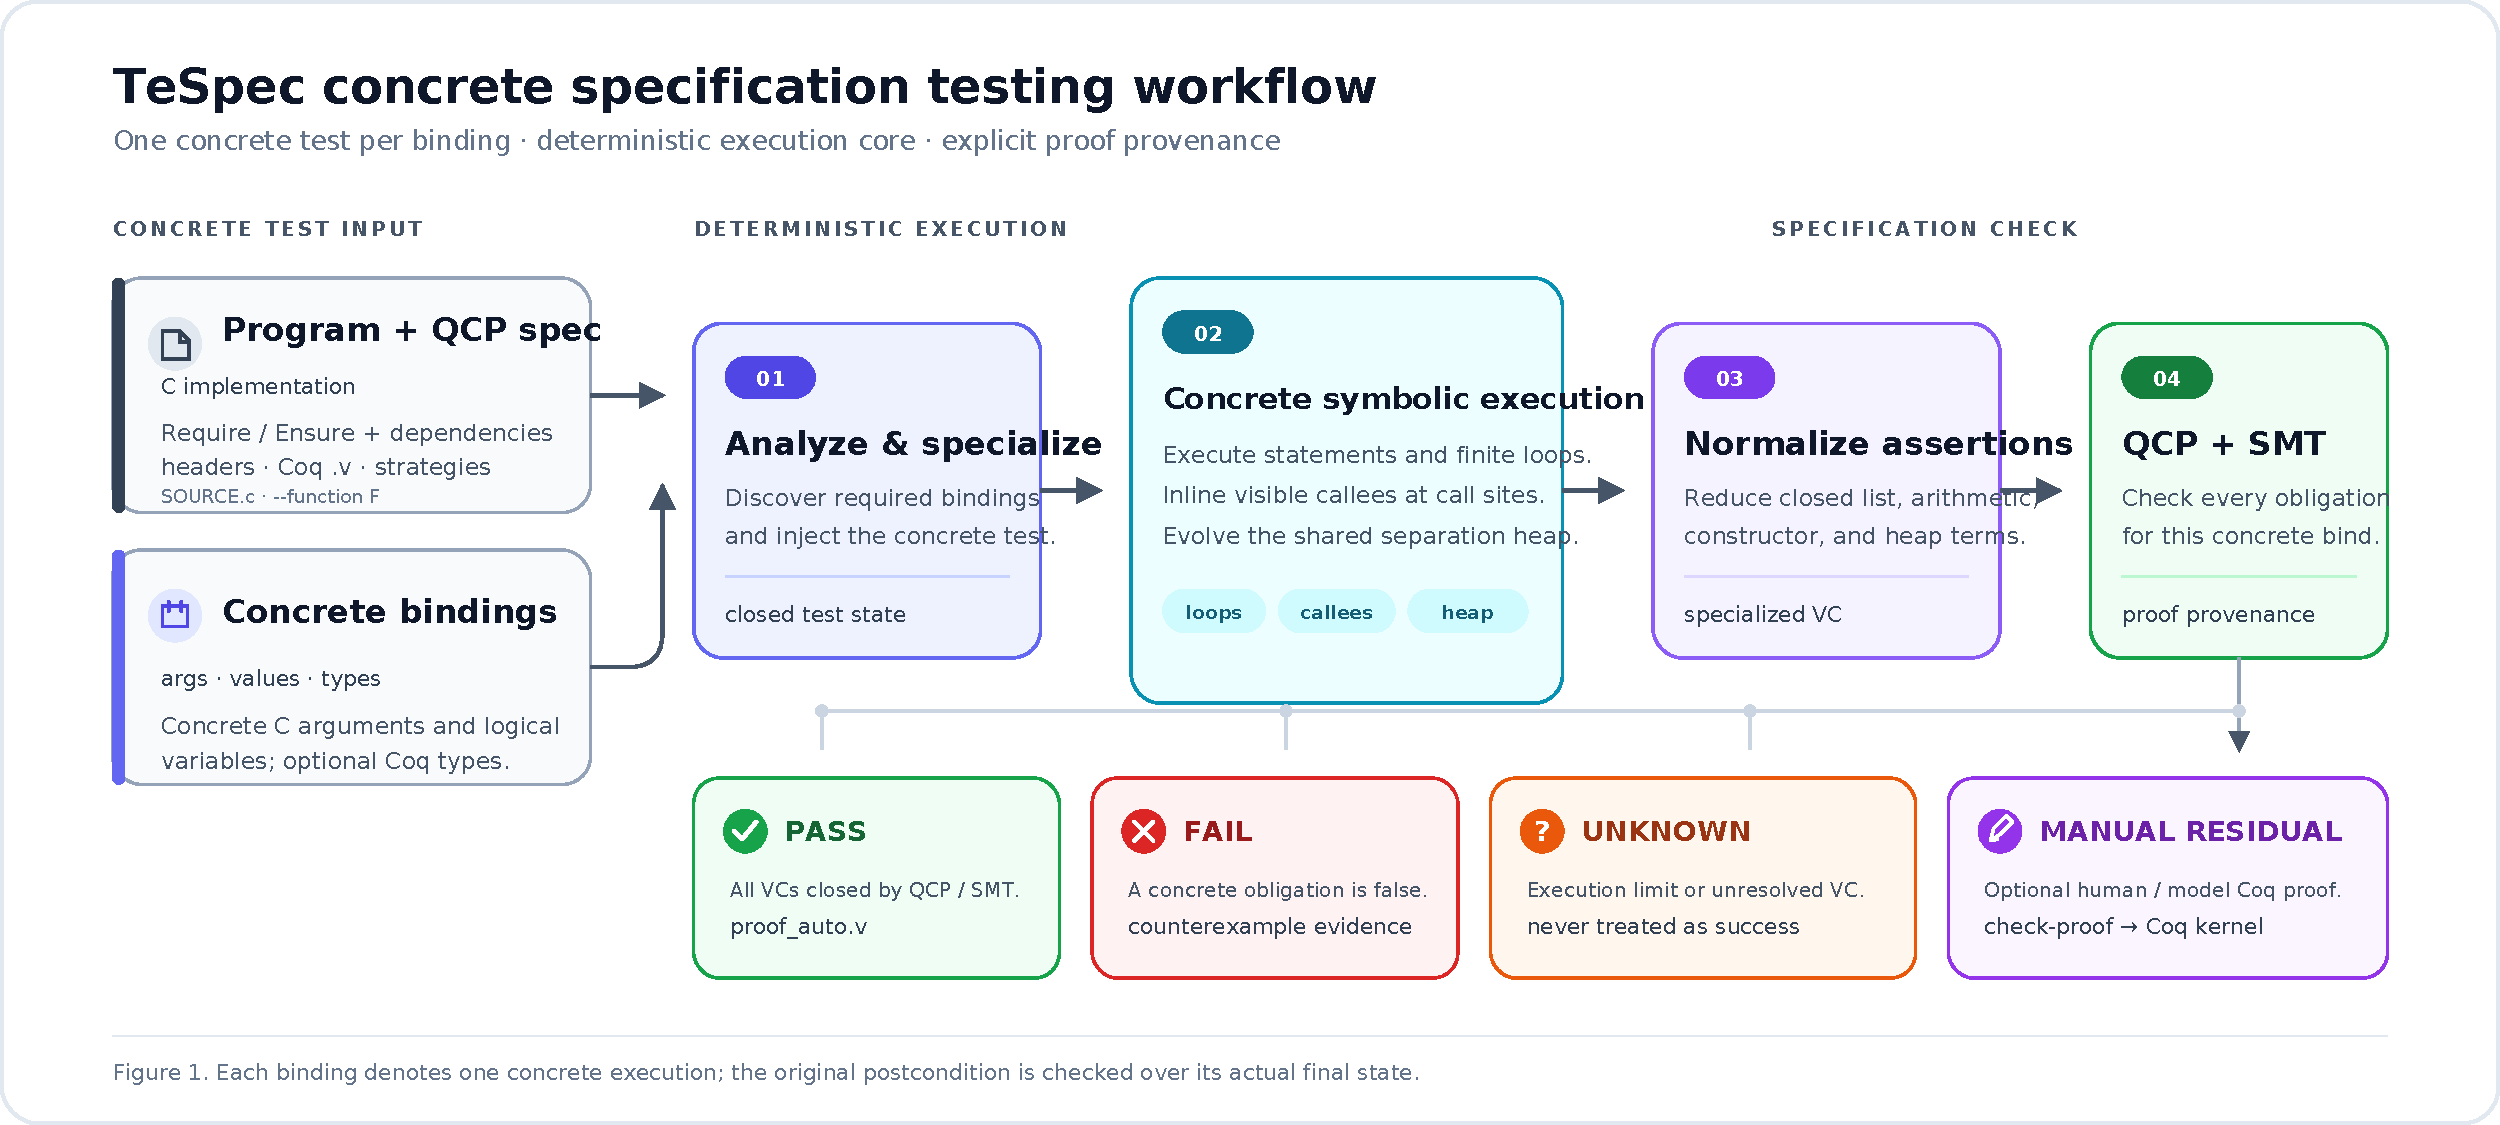
\includegraphics[width=\linewidth]{../docs/assets/tespec-workflow.pdf}
  \caption{\tespec{} workflow.  The agent-facing binding and residual-proof
  steps propose artifacts; parsing, execution, proof generation, and verdict
  classification remain deterministic.}
  \label{fig:workflow}
\end{figure}

\tespec{} accepts:

\[
\texttt{QCP contract + C implementation + one or more binds}.
\]

A bind record describes:

\begin{itemize}[leftmargin=1.4em]
  \item the target function;
  \item concrete scalar and pointer arguments;
  \item arrays, structures, globals, and allocated heap blocks reachable from
        pointer roots;
  \item values for \texttt{With} variables; and
  \item execution limits and task-local logical dependencies.
\end{itemize}

The interface separates semantic evidence from execution diagnostics.  Under
the strict evidence policy below, a selected contract instance is satisfied,
violated, or unresolved.  Parsing and dependency errors, incomplete heap
descriptions, exhausted execution bounds, safety failures, and unproved QCP
inconsistencies are reported separately and are not silently promoted to
semantic verdicts.

\subsection{A lightweight case model}

We use a small amount of notation to make the engineering contract precise.
A concrete behavior is:
\[
  b=(a,H_0,r,H_1),
\]
where \(a\) contains C arguments, \(H_0\) and \(H_1\) are finite typed heaps,
and \(r\) is the return value.  A bind \(\eta\) assigns values to the
\texttt{With} variables of the selected QCP specification.

After substitution, a precondition or postcondition becomes a closed
proposition:
\[
  \phi=\mathsf{instantiate}(S,\eta,a,H_0,r,H_1).
\]
The testing workflow uses three outcomes:
\[
\begin{array}{ll}
\pass & \text{a checked proof of the expected proposition is available},\\
\fail & \text{a checked proof of its opposite is available},\\
\unknown & \text{neither direction was established within the budget}.
\end{array}
\]
This is an operational evidence policy, not a new program logic.  In
particular, failure of SMT or symbolic execution is not by itself evidence
that a specification is false.

Each bind selects one indexed contract instance.  This is analogous to a
parameterized unit/property test: the result does not claim anything about
unseen bindings.  Comparative specification evaluation should reuse the same
frozen heap cases and binding schema across candidates; interactive use may
allow the candidate precondition to materialize its own heap, but such results
must not be compared as if they used identical inputs.

\section{Approach}

\subsection{Step 1: discover the testing interface}

The analyzer parses the C signature and QCP annotations, then reports:

\begin{itemize}[leftmargin=1.4em]
  \item ordinary C parameters and their scalar/pointer types;
  \item value-level and type-level \texttt{With} declarations;
  \item referenced globals and spatial predicates;
  \item task-local \texttt{Import Coq}, \texttt{Extern Coq}, and strategy
        dependencies; and
  \item heap regions that the precondition can use to initialize execution.
\end{itemize}

The generated bind template is intentionally typed rather than program
specific.  It supports integers, machine scalars, nested lists, constructor
terms, arrays, closed structures, pointer roots, and a raw QCP/Rocq term escape
hatch for application-defined types.  The same representation composes: an
array cell may contain a structure, a structure may contain list roots, and a
list node may contain arrays or closed substructures.

\subsection{Step 2: construct and freeze the initial state}

In interactive mode, the tool combines the bind with the spatial
\texttt{Require} to allocate fresh blocks and initialize cells.  Pointers are
represented internally as block-offset pairs, preserving aliases without
depending on process-specific addresses.

The planned publication mode exports the resulting initial state as a case
record and replays it independently of the candidate specification.  This
avoids a
candidate-controlled-input problem: two specifications must not receive
different list lengths merely because their preconditions materialize
different heaps.

All memory required by execution must be concrete.  A symbolic frame may be
retained for untouched regions during interactive execution, but a comparative
case must also fix memory observable by the candidate contract.  The evaluator
records which cells were read, written, or only framed to make this distinction
auditable.

\subsection{Step 3: follow the concrete execution}

The modified QCP executor preserves the ordinary spatial reasoning needed for
loads and stores, but uses concrete values to choose the path.

\paragraph{Branches.}
An encountered condition must reduce to a concrete Boolean.  If it does not,
the case is incomplete and returns \unknown{} rather than exploring an
arbitrary branch.

\paragraph{Loops.}
The executor repeatedly evaluates the guard and body until the concrete guard
becomes false.  \texttt{break}, \texttt{continue}, and \texttt{return} retain
their QCP control-flow meanings.  A global iteration limit prevents accidental
divergence; exhausting it returns \unknown.  No loop invariant is requested
because the tool records one finite run rather than proving all iterations.

\paragraph{Visible calls.}
For a call whose body is available, the executor evaluates actual arguments,
creates a fresh local frame, executes the callee, propagates the return value
and shared heap, and resumes the caller.  It therefore does not need a callee
contract or callee ghost bind for that call.  Opaque external functions require
an explicit task-local model.

\paragraph{Safety.}
Concrete mode does not skip pointer validity, ownership, bounds, or definedness
checks.  Knowing a numeric address is not the same as owning a valid cell.
Failure to derive the spatial resource is reported as an execution/safety
failure, not automatically as a failed terminal specification.

\subsection{Step 4: specialize and simplify the contract}

At the target function boundary, \tespec{} substitutes:

\[
  \eta,\quad a,\quad H_0,\quad r,\quad H_1
\]
into the selected \texttt{Require} or \texttt{Ensure}.  The source assertion is
preserved; the tool does not synthesize a separate executable checker.

Generic simplification reduces closed arithmetic, Boolean expressions,
constructor matches, list length/indexing, known recursive calls, and concrete
spatial atoms.  Simplification rules operate on typed AST forms rather than
function names or benchmark constants.  Unsupported constructs remain in the
goal.

\subsection{Step 5: discharge and report}

The backend follows QCP's normal artifact split:

\begin{itemize}[leftmargin=1.4em]
  \item a goal file containing generated VCs;
  \item automatic proofs produced by spatial strategies and SMT;
  \item a residual proof file for unresolved goals; and
  \item a final Rocq module that checks proof coverage.
\end{itemize}

QCP's SMT layer is effective for closed linear arithmetic and uninterpreted
functions, but arbitrary quantified or domain-specific propositions may remain
residual.  A proof agent may propose a proof script, but the script is accepted
only if Rocq compiles it against the original goal.  Agent failure leaves the
case unresolved.

\section{Binding as a User and Agent Interface}

Logical binding is often the least familiar part of the workflow.  The C run
may show a three-node heap, while the contract expects a \texttt{list Z}, a
nested constructor, or an application-specific Rocq value.  \tespec{} separates
three activities:

\begin{enumerate}[leftmargin=1.4em]
  \item \textbf{Discovery:} deterministic analysis reports all values that must
        be supplied and their types.
  \item \textbf{Proposal:} a user or agent fills the template using the
        pre-state, source contract, and task-local definitions.
  \item \textbf{Checking:} the deterministic core parses, type-checks, and
        applies the binding; a malformed proposal cannot change the verdict.
\end{enumerate}

The accompanying Codex skill documents how to inspect the initial heap, map
recursive predicates to logical values, run the tool, and handle residual VCs.
The skill is a usability layer rather than a component of the semantic oracle.
To prevent output leakage, a binding for a pre-state is saved before examining
the final heap and reused for positive and mutant executions from that state.

Human-authored binds remain first-class.  Every agent-produced bind is stored
as ordinary input data, making the run reproducible without the original
conversation or model.

\section{Implementation}

The prototype is packaged independently under \texttt{specTest}.  Each case
stores its C source, binds, Rocq definitions, QCP strategies, and generated
evidence locally; it does not depend on a monolithic external case corpus.

The implementation has four main components:

\begin{description}[leftmargin=1.35in,style=nextline]
  \item[Analyzer] Parses function signatures, QCP contracts, imports, and
        logical-variable declarations and emits a bind template.
  \item[Case builder] Creates typed heap blocks and globals from the binding or
        replays a frozen case.
  \item[Concrete executor] Extends QCP with finite loop execution, visible-call
        inlining, concrete branch selection, and resource limits.
  \item[Evidence backend] Specializes the boundary assertion, runs generic
        reductions, invokes QCP/SMT, and packages automatic and residual Rocq
        proof files.
\end{description}

\subsection{Supported program shapes}

The present engineering target is deterministic sequential C with:

\begin{itemize}[leftmargin=1.4em]
  \item primitive scalars and supported opaque 64-bit cells;
  \item arrays and arrays of closed structures;
  \item nested closed structures and globals;
  \item singly and doubly linked lists;
  \item recursive combinations of arrays, structures, and list nodes;
  \item finite loops, nested loops, visible calls, and bounded recursion; and
  \item QCP \texttt{Let} predicates and task-local transparent Rocq
        definitions.
\end{itemize}

Trees, unrestricted graphs, concurrency, function pointers, \texttt{goto},
volatile/device effects, and unsupported floating semantics are outside the
current claim.  They produce an explicit unsupported or unresolved result
unless a trusted case-local model is supplied.

\subsection{Prototype and publication-mode distinction}

The current command-line workflow is already useful for testing a supplied
contract against a self-materialized execution.  A comparative
specification-evaluation experiment requires additional controls:

\begin{itemize}[leftmargin=1.4em]
  \item freeze candidate-independent initial heaps;
  \item use the same bind schema and cases across candidate specifications;
  \item certify positive and negative labels independently;
  \item distinguish execution/safety diagnostics from terminal-contract
        violations; and
  \item require a checked opposite-polarity goal for a conclusive
        \fail{} result.
\end{itemize}

These controls define a strict \emph{evaluation mode}; they are not all
implemented by the current diagnostic prototype.  In particular, the current
CLI can surface a QCP-reported inconsistent obligation, but the paper reserves
\fail{} for a separately generated and checked opposite-polarity proposition.
Diagnostic-only failures must therefore remain outside semantic rejection
counts.

\section{Benchmark Design}
\label{sec:evaluation}

\subsection{A four-class task without supplied test cases}

The benchmark evaluates whether an LLM or agent can classify a candidate
contract, rather than whether it can answer a preselected instance.  A
question exposes exactly one implementation \(I\) and one QCP contract \(S\).
It does \emph{not} provide concrete test inputs, parent implementations, or
mutation metadata.  Mutation relationships between questions are hidden
construction lineage and cannot substitute for evidence about the current
pair.  A subject that predicts a negative property must discover and submit
its own C arguments, initial heap, and logical bindings as a checkable
counterexample.

For a legal typed state \(x=(a,H_0)\), let \(B(I,x)\) be the safely terminating
observable behavior, including return value, canonical final heap, modeled
globals, and external-call events.  Let \(R_I\) contain all
\((x,B(I,x))\), and let \(R_S\) contain all \((x,y)\) admitted by the
contract's \texttt{Require} and \texttt{Ensure} under logical bindings frozen
from the initial state.  We define:
\[
\begin{split}
\mathsf{Sound}(S,I) &\triangleq R_S\subseteq R_I,\\
\mathsf{Complete}(S,I) &\triangleq R_I\subseteq R_S.
\end{split}
\]
Thus soundness says that the specification admits no behavior the
implementation cannot produce, while completeness says that it omits no
defined implementation behavior.  The first benchmark version is
deterministic and sequential.

\begin{center}
\small
\begin{tabular}{lccp{0.47\linewidth}}
\toprule
label & Sound & Complete & interpretation\\
\midrule
\textsf{CORRECT}      & yes & yes & equals the implementation behavior
                                         relation\\
\textsf{SOUNDNESS}    & yes & no  & is too strong and omits some
                                         implementation behavior\\
\textsf{COMPLETE}     & no  & yes & is too weak and admits behavior the
                                         implementation cannot produce\\
\textsf{INCOMPARABLE} & no  & no  & both omits implementation behavior and
                                         admits non-implementation behavior\\
\bottomrule
\end{tabular}
\end{center}

The class names \textsf{SOUNDNESS} and \textsf{COMPLETE} mean sound-only and
complete-only in this table.  We give the formulas because prior work uses
these words in both inclusion directions.

\subsection{Counterexample certificates}

A soundness counterexample is a checked witness
\[
  (x,y)\in R_S\setminus R_I.
\]
A completeness counterexample is a checked witness
\[
  (x,B(I,x))\in R_I\setminus R_S.
\]
Both certificates contain concrete C arguments, the complete relevant initial
heap, pre-state logical bindings, and checked candidate polarity.  A
soundness counterexample additionally proves that the admitted behavior is
not the implementation behavior; a completeness counterexample archives the
implementation trace and the candidate rejection.  We exclude undefined,
crashing, nonterminating, and unmodeled-I/O executions from semantic evidence.

The benchmark has binary gold values for the two properties, but an evaluated
tool may abstain.  Failure to find a counterexample never establishes a
positive property.  Gold \textsf{yes} axes therefore require a checked
inclusion proof (or an explicitly complete finite-domain certificate), while
gold \textsf{no} axes require the counterexamples above.

\subsection{One hundred programs and six questions each}

We shortlist 100 difficult annotated target functions and construct six
implementation/specification questions per function, for 600 questions.
Every base contributes at least one question from each class, three
\emph{hard} questions, and three \emph{expert} questions.  The two additional
class occurrences rotate across bases, yielding exactly 150 questions per
class, with 75 in each class/difficulty cell.
Hard items require at least one semantic specification transformation and two
reasoning dimensions.  Expert items require at least two sequential,
nonredundant transformations, surface camouflage, and three reasoning
dimensions.

The subject pool deliberately combines arrays, strings, closed structures,
singly and doubly linked lists, nested control flow, visible calls, native
floating-point operations, floating-point models, quantifiers, and custom
Rocq definitions.  Selection occurs at the target-function level, but all
targets from one source family remain in one data split.

Mutation recipes include equivalent fold/unfold and logical rewrites;
weakenings that omit return, heap, ordering, quantifier, call-event, or
link-consistency constraints; strengthenings that overconstrain an input,
return, heap cell, floating result, or list relation; and mixed mutations for
the incomparable class.  Implementation mutations cover branches, loop
bounds, indices, writes, fields, calls, floating operators, and list links.
An operator name does not determine a label: redundant edits and equivalent
mutants are discarded after semantic auditing.

\subsection{Gold construction, difficulty, and leakage control}

For implementation relation \(R_I\) and candidate relation \(R_S\), a correct
item stores proofs of both inclusions.  A sound-only item stores
\(R_S\subseteq R_I\) and an implementation-only witness.  A complete-only item
stores \(R_I\subseteq R_S\) and a specification-only witness.  An incomparable
item stores both witnesses.  Each item also archives source and dependency
hashes, canonical heaps and traces, selected QCP specification,
binding-adequacy evidence, normalized propositions, proof polarity, and
checker version.

Difficulty scores reject obviously shallow construction plans but are not
the authoritative difficulty criterion.  Each materialized question receives
three independent runs of the frozen OpenHands plus
\texttt{openai/gpt-5-nano} generic-agent baseline.  We retain questions solved
in at most one run and replace questions solved in at least two runs with a
fresh question of the same class.  Infrastructure failures remain unresolved
rather than counting as model errors.  A scored trajectory must also attest
that the agent inspected both public semantic inputs; a label emitted without
reading either input is unresolved.  Release additionally requires this Nano
gate, a difficulty-gate certificate, balanced surface-statistics audit,
label-blind mutation review, and, for expert items, a composed-mutation
nonredundancy certificate.

The train/development/test split is grouped by project, source family, and
predicate family; all six questions for a base program stay together.
Mutation and label names are removed from the model-visible package.  We
balance edit size and contract length across classes and hold out mutation
families to test whether a model learned semantics rather than the generator's
surface pattern.

\subsection{Model and tool comparison}

We use a paired protocol for each model:

\begin{enumerate}[leftmargin=1.4em]
  \item direct LLM classification from the source package;
  \item a generic coding agent with ordinary repository and shell tools; and
  \item the same agent and budget with the \tespec{} skill and CLI available.
\end{enumerate}

The third condition may use \tespec{} to analyze bindings, execute the
implementation, replay canonical heaps, and check both candidate proposition
polarities.  The tool does not receive the hidden class and does not emit the
four-way answer.  We report four-class accuracy and macro-F1, balanced
accuracy on each Boolean axis, and \emph{certificate success}, which requires
both the correct label and valid counterexamples for every predicted-false
axis.  Cost, time, calls, abstention, proof provenance, and feature-stratified
results are secondary metrics.  Confidence intervals use a
base-program-clustered bootstrap because six questions from one program are not
independent observations.

\subsection{Empirical results}

\noindent\textit{The empirical results are intentionally left blank in this
draft.  They will be populated only after all 600 questions pass the frozen
gold audit; the static shortlist and internal regression runs are not reported
as benchmark results.}

\section{Engineering Assurances}

\tespec{} does not introduce a new proof calculus.  Its evidence chain reuses
QCP's generated-goal, automatic-proof, residual-proof, and final-check module
architecture.  The Rocq check establishes that each listed goal has a proof;
it does not validate a buggy frontend or an omitted VC.  We therefore adopt the
following engineering controls:

\begin{itemize}[leftmargin=1.4em]
  \item archive the exact source, bind, heap, generated goal, proof files, tool
        versions, and hashes for every result;
  \item prohibit \texttt{Admitted}, candidate-supplied axioms, and proof escape
        hatches;
  \item compile the final proof-check module for every proof-backed verdict;
  \item never classify prover failure as semantic rejection;
  \item run differential checks between native execution and concrete QCP
        execution on the supported C subset;
  \item test generic reductions with name- and constant-renamed programs; and
  \item maintain held-out projects and predicate families to detect
        case-specific patches.
\end{itemize}

These controls support reproducibility and reduce false conclusions, but they
are not presented as a mechanized end-to-end soundness theorem for the modified
executor.

\section{Threats to Validity}

\paragraph{Construct validity.}
Passing finite cases measures agreement with those cases, not universal
specification correctness.  Mutation score depends on the chosen fault model,
and automatically generated mutants may be equivalent.  We mitigate these
issues by separating positive/negative pre/post results, reviewing mutation
operators, and reporting uncertified cases.

\paragraph{Internal validity.}
Incorrect binds, heap replay, reference contracts, or case labels could bias
the result.  We store all intermediate artifacts, reuse frozen inputs across
candidates, validate binds independently, and require proof-backed labels for
the strict experiment.

\paragraph{External validity.}
QCP and QCIP/CAV subjects may not represent all systems C.  The current scope
excludes concurrency, graphs, device memory, and several C features.  We report
results by feature and use held-out projects instead of extrapolating from one
corpus.

\paragraph{Conclusion validity.}
Proof-search timeouts can make a true instance appear unresolved.  We keep
\unknown{} separate from rejection, report lower and upper resolution bounds,
repeat stochastic agent conditions, and use paired analyses for ablations.

\paragraph{Agent and data leakage.}
An LLM may have seen public examples or infer a bind from output information.
We use held-out transformations and projects, prevent the binding step from
seeing terminal states, archive prompts, and report human-only and
agent-assisted settings separately.

\section{Related Work}

Table~\ref{tab:related} summarizes the closest design points.  The categories
describe the default workflow of each system; they are not claims that a
framework could never be extended.

\begin{table}[t]
\centering
\small
\begin{tabular}{p{.20\linewidth}p{.16\linewidth}p{.18\linewidth}p{.34\linewidth}}
\toprule
Approach & Cases & Native C heap & Test oracle\\
\midrule
QuickCheck / QuickChick
  & Generated values & No mutable C ownership
  & Executable property\\
Fulminate
  & Supplied executions & Yes
  & Compiled runtime checks for CN\\
Bennet
  & Generated heaps & Yes
  & Generated CN runtime checks\\
VERINA / COINS
  & Fixed positive/negative values & No native C heap transition
  & Tests and/or proof-checked proposition\\
\tespec
  & Supplied typed heaps and binds & Yes
  & Specialized QCP/Rocq proof obligation\\
\bottomrule
\end{tabular}
\caption{Design-space comparison with representative related systems.}
\label{tab:related}
\end{table}

\subsection{Property-based testing}

QuickCheck popularized testing executable properties over generated inputs
~\citep{claessen2000quickcheck}.
Subsequent PBT systems improved generation, shrinking, and integration with
proof assistants.  QuickChick provides a foundational PBT framework for Coq
developments~\citep{paraskevopoulou2015quickchick}; FuzzChick combines
property-based generation with coverage-guided mutation to reach behavior
hidden behind sparse semantic preconditions~\citep{lampropoulos2019fuzzchick}.
These systems treat the property as an executable decision procedure.  In
contrast, \tespec{} treats the test oracle as a closed proof obligation, which
accepts proof-oriented predicates for which no executable checker is supplied,
but is necessarily more expensive and may return a residual goal.

PBT research also highlights that generating valid structured inputs is often
harder than running the property.  \tespec{} currently consumes explicit typed
bindings rather than claiming a complete random generator.  Its bind analyzer
and optional agent address authoring effort, while input generation and
shrinking remain complementary future work.

\subsection{Testing heap specifications}

Runtime checking and test generation for heap-manipulating programs are the
closest technical relatives.  SLICK explored runtime checking of
separation-logic invariants~\citep{nguyen2008slick}.  CSF uses
separation-logic preconditions in concolic test generation
~\citep{pham2019csf}.  Fulminate compiles CN specifications to instrumented C
and checks ownership transfer at runtime~\citep{banerjee2025fulminate}.
Bennet builds on the same executable CN fragment to synthesize backtracking
generators for complex heap inputs~\citep{aamer2025bennet}.

This line of work invalidates any broad claim that PBT cannot handle heaps.
The meaningful distinction is expressiveness and oracle construction.
Fulminate and Bennet intentionally exploit a restricted presentation of
separation logic with an effective computational interpretation.  \tespec{}
targets existing QCP specifications that may contain application-defined
transparent Rocq definitions, quantified propositions, and residual proof
obligations.
It follows one supplied heap case and proves the instantiated assertion instead
of compiling all supported assertions into runtime code.

\subsection{Formal specification evaluation}

FormalBench studies specification inference through consistency and
completeness and uses mutation-oriented analysis to expose semantic weaknesses
~\citep{lecong2025formalbench}.  CLEVER evaluates generated Lean
specifications against curated references with formal equivalence
~\citep{thakur2025clever}.  VERINA decomposes verifiable-code generation into
code, specification, and proof tasks, and evaluates specifications with
positive and negative test suites~\citep{ye2026verina}.  COINS directly proves
specialized declarative specifications on concrete value-level examples
~\citep{yang2026coins}.  VeriScale expands test suites with adversarial
implementations and then reduces them while preserving discriminative power
~\citep{bai2026veriscale}.  OSVBench broadens specification generation to
operating-system verification tasks~\citep{li2026osvbench}.  MutDafny uses
implementation mutation to identify weak Dafny specifications and derives
language-specific operators from real bug-fix commits
~\citep{amaral2026mutdafny}.

\tespec{} adopts the central testing insight of this work: desired behaviors
measure over-restriction, while undesired behaviors measure
under-specification.  Its contribution is an engineering path for applying
that idea to mutable C heap transitions and QCP separation-logic contracts.
Unlike reference-equivalence evaluation, it does not attempt to prove two
contracts universally equivalent.  Unlike purely value-level instance
evaluation, a case includes typed memory, aliasing, global state, and old/new
heap contents.

\subsection{Verification and agentic assistance}

QCP provides the verification infrastructure reused by \tespec: symbolic
execution, a separation-logic entailment solver, SMT, and residual Rocq proofs
~\citep{wu2026qcp}.  Standard QCP targets universal function verification;
\tespec{} specializes this machinery to selected concrete cases for debugging
and evaluation.

Recent work explores agents for separation-logic specification synthesis and
program verification~\citep{suresh2026agentic}.  \tespec{} uses an agent only
as an optional interface for proposing binds and residual proofs.  This role
separation is methodologically important: agent success affects automation and
cost, while deterministic parsers, execution, and proof checking determine the
recorded evidence.

\section{Discussion}

\paragraph{A complement to PBT, not a replacement.}
When a contract has a faithful executable interpretation, compiled PBT offers
orders-of-magnitude more cases and mature shrinking.  \tespec{} is intended for
the remaining assertions: those already written for deductive verification
whose logical expressiveness prevents direct execution.  A practical workflow
can use both, routing executable fragments to runtime testing and difficult
closed instances to proof-backed checking.

\paragraph{Testing the specification versus testing the implementation.}
The same execution can serve two purposes.  With a trusted contract, mutants
test an implementation.  With trusted positive and negative behaviors, the
behaviors test a candidate contract.  A future evaluation will use the latter
view: the implementation generates heap transitions, while the candidate
specification is the artifact being assessed.  The evaluation section remains
unpopulated in this draft.

\paragraph{Why concrete symbolic execution?}
Native execution alone produces bytes and addresses but not the QCP spatial
state needed to instantiate the contract.  Universal QCP verification requires
invariants and callee contracts that are unnecessary for one test.  Concrete
symbolic execution occupies the middle: it follows one path while retaining
the assertion and heap representation expected by the QCP backend.

\paragraph{Where agents add value.}
Mapping an arbitrary recursive heap to an arbitrary Rocq type and proving a
domain-specific residual are open-ended tasks.  Agents are useful proposal
mechanisms for both, but the core tool remains usable with human-authored binds
and proofs.  Keeping agent artifacts explicit also enables controlled
experiments rather than treating an LLM as an unobservable judge.

\section{Conclusion}

\tespec{} brings test-style feedback to expressive QCP specifications for
heap-manipulating C.  Users provide concrete program inputs and typed logical
bindings; the tool follows finite loops and visible calls, records the heap
transition, specializes the original contract, and invokes QCP/SMT/Rocq to
check the resulting instance.  The design complements executable PBT systems
such as Fulminate and Bennet and extends instance-based specification
evaluation from ordinary values to arrays, structures, aliasing, and linked
heaps.

The design claim is deliberately engineering-oriented: \tespec{} should
eventually be judged by the QCP contracts it can exercise, the fraction of
instances it resolves automatically, the specification faults its positive
and negative cases expose, and the effort required to supply binds.  This
draft reports none of those measurements.  The approach does not turn finite
testing into universal verification, but provides a path toward reproducible,
proof-backed debugging of contracts that do not come with runtime checkers.

\bibliographystyle{plainnat}
\bibliography{references}

\end{document}
